\documentclass[tikz, border=10pt]{standalone}
\usepackage{tikz}
\usetikzlibrary{shapes, positioning, arrows.meta, calc, backgrounds}

\begin{document}
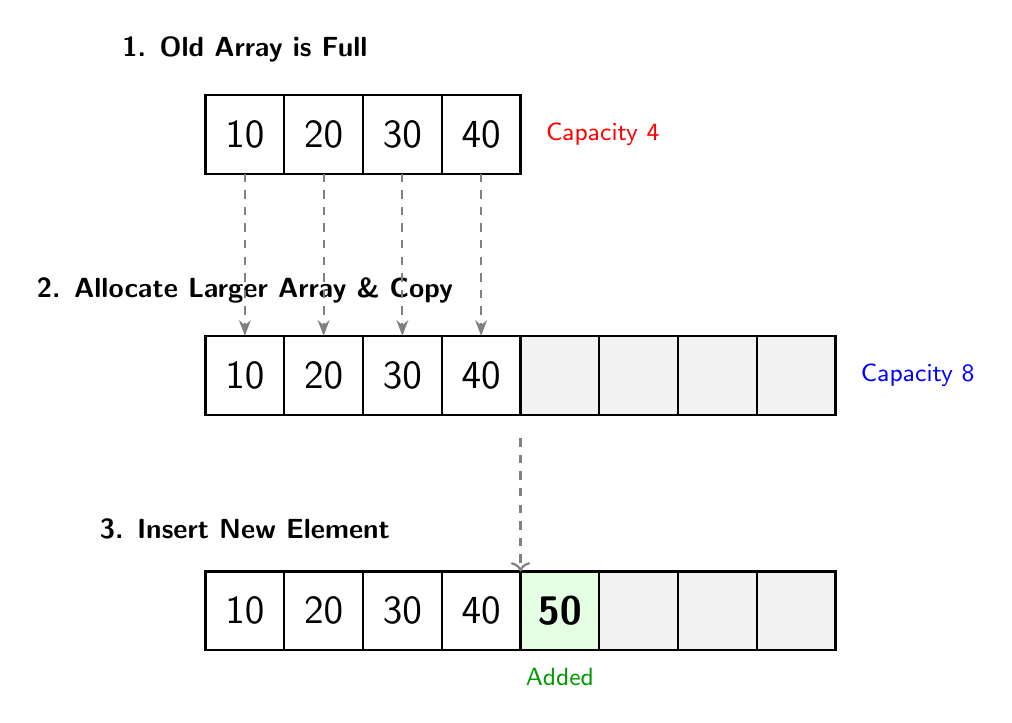
\begin{tikzpicture}[
    cell/.style={
        rectangle, 
        draw=black, 
        thick, 
        minimum width=1cm, 
        minimum height=1cm, 
        node distance=0cm, 
        outer sep=0pt,
        font=\Large\sffamily
    },
    index/.style={
        font=\small\ttfamily\color{gray},
        below=0.1cm of #1
    },
    arrow/.style={
        ->, 
        thick, 
        color=blue, 
        >={Stealth[length=2mm]},
        dashed
    },
    label_text/.style={
        font=\sffamily\bfseries
    }
]

    % -- Step 1: Old Array (Full) --
    \node[label_text] (label_step1) {1. Old Array is Full};
    
    \node[cell, below=0.3cm of label_step1] (old0) {10};
    \node[cell, right=of old0] (old1) {20};
    \node[cell, right=of old1] (old2) {30};
    \node[cell, right=of old2] (old3) {40};
    \node[right=0.2cm of old3, color=red, font=\small\sffamily] {Capacity 4};

    % -- Step 2: Allocate & Copy --
    \node[label_text, below=1.2cm of old0] (label_step2) {2. Allocate Larger Array \& Copy};

    \node[cell, below=0.3cm of label_step2] (copy0) {10};
    \node[cell, right=of copy0] (copy1) {20};
    \node[cell, right=of copy1] (copy2) {30};
    \node[cell, right=of copy2] (copy3) {40};
    \node[cell, right=of copy3, fill=gray!10] (copy4) {};
    \node[cell, right=of copy4, fill=gray!10] (copy5) {};
    \node[cell, right=of copy5, fill=gray!10] (copy6) {};
    \node[cell, right=of copy6, fill=gray!10] (copy7) {};
    \node[right=0.2cm of copy7, color=blue, font=\small\sffamily] {Capacity 8};

    % Arrows showing copying
    \draw[arrow, gray] (old0.south) -- (copy0.north);
    \draw[arrow, gray] (old1.south) -- (copy1.north);
    \draw[arrow, gray] (old2.south) -- (copy2.north);
    \draw[arrow, gray] (old3.south) -- (copy3.north);


    % -- Step 3: Insert New Element --
    \node[label_text, below=1.2cm of copy0] (label_step3) {3. Insert New Element};

    \node[cell, below=0.3cm of label_step3] (new0) {10};
    \node[cell, right=of new0] (new1) {20};
    \node[cell, right=of new1] (new2) {30};
    \node[cell, right=of new2] (new3) {40};
    \node[cell, right=of new3, fill=green!10] (new4) {\textbf{50}}; % New insertion
    \node[cell, right=of new4, fill=gray!10] (new5) {};
    \node[cell, right=of new5, fill=gray!10] (new6) {};
    \node[cell, right=of new6, fill=gray!10] (new7) {};

    \node[below=0.1cm of new4, color=green!60!black, font=\small\sffamily] {Added};

    % Transition Arrow Step 2 -> 3
    \draw[->, thick, gray, dashed] ($(copy3.south east)!0.5!(copy4.south west)$) ++(0, -0.3) -- ($(new3.north east)!0.5!(new4.north west)$);


\end{tikzpicture}
\end{document}
